\documentclass[twoside]{book}

% Packages required by doxygen
\usepackage{fixltx2e}
\usepackage{calc}
\usepackage{doxygen}
\usepackage[export]{adjustbox} % also loads graphicx
\usepackage{graphicx}
\usepackage[utf8]{inputenc}
\usepackage{makeidx}
\usepackage{multicol}
\usepackage{multirow}
\PassOptionsToPackage{warn}{textcomp}
\usepackage{textcomp}
\usepackage[nointegrals]{wasysym}
\usepackage[table]{xcolor}

% Font selection
\usepackage[T1]{fontenc}
\usepackage[scaled=.90]{helvet}
\usepackage{courier}
\usepackage{amssymb}
\usepackage{sectsty}
\renewcommand{\familydefault}{\sfdefault}
\allsectionsfont{%
  \fontseries{bc}\selectfont%
  \color{darkgray}%
}
\renewcommand{\DoxyLabelFont}{%
  \fontseries{bc}\selectfont%
  \color{darkgray}%
}
\newcommand{\+}{\discretionary{\mbox{\scriptsize$\hookleftarrow$}}{}{}}

% Page & text layout
\usepackage{geometry}
\geometry{%
  a4paper,%
  top=2.5cm,%
  bottom=2.5cm,%
  left=2.5cm,%
  right=2.5cm%
}
\tolerance=750
\hfuzz=15pt
\hbadness=750
\setlength{\emergencystretch}{15pt}
\setlength{\parindent}{0cm}
\setlength{\parskip}{3ex plus 2ex minus 2ex}
\makeatletter
\renewcommand{\paragraph}{%
  \@startsection{paragraph}{4}{0ex}{-1.0ex}{1.0ex}{%
    \normalfont\normalsize\bfseries\SS@parafont%
  }%
}
\renewcommand{\subparagraph}{%
  \@startsection{subparagraph}{5}{0ex}{-1.0ex}{1.0ex}{%
    \normalfont\normalsize\bfseries\SS@subparafont%
  }%
}
\makeatother

% Headers & footers
\usepackage{fancyhdr}
\pagestyle{fancyplain}
\fancyhead[LE]{\fancyplain{}{\bfseries\thepage}}
\fancyhead[CE]{\fancyplain{}{}}
\fancyhead[RE]{\fancyplain{}{\bfseries\leftmark}}
\fancyhead[LO]{\fancyplain{}{\bfseries\rightmark}}
\fancyhead[CO]{\fancyplain{}{}}
\fancyhead[RO]{\fancyplain{}{\bfseries\thepage}}
\fancyfoot[LE]{\fancyplain{}{}}
\fancyfoot[CE]{\fancyplain{}{}}
\fancyfoot[RE]{\fancyplain{}{\bfseries\scriptsize Generated by Doxygen }}
\fancyfoot[LO]{\fancyplain{}{\bfseries\scriptsize Generated by Doxygen }}
\fancyfoot[CO]{\fancyplain{}{}}
\fancyfoot[RO]{\fancyplain{}{}}
\renewcommand{\footrulewidth}{0.4pt}
\renewcommand{\chaptermark}[1]{%
  \markboth{#1}{}%
}
\renewcommand{\sectionmark}[1]{%
  \markright{\thesection\ #1}%
}

% Indices & bibliography
\usepackage{natbib}
\usepackage[titles]{tocloft}
\setcounter{tocdepth}{3}
\setcounter{secnumdepth}{5}
\makeindex

% Hyperlinks (required, but should be loaded last)
\usepackage{ifpdf}
\ifpdf
  \usepackage[pdftex,pagebackref=true]{hyperref}
\else
  \usepackage[ps2pdf,pagebackref=true]{hyperref}
\fi
\hypersetup{%
  colorlinks=true,%
  linkcolor=blue,%
  citecolor=blue,%
  unicode%
}

% Custom commands
\newcommand{\clearemptydoublepage}{%
  \newpage{\pagestyle{empty}\cleardoublepage}%
}

\usepackage{caption}
\captionsetup{labelsep=space,justification=centering,font={bf},singlelinecheck=off,skip=4pt,position=top}

%===== C O N T E N T S =====

\begin{document}

% Titlepage & ToC
\hypersetup{pageanchor=false,
             bookmarksnumbered=true,
             pdfencoding=unicode
            }
\pagenumbering{roman}
\begin{titlepage}
\vspace*{7cm}
\begin{center}%
{\Large My Project }\\
\vspace*{1cm}
{\large Generated by Doxygen 1.8.11}\\
\end{center}
\end{titlepage}
\clearemptydoublepage
\tableofcontents
\clearemptydoublepage
\pagenumbering{arabic}
\hypersetup{pageanchor=true}

%--- Begin generated contents ---
\chapter{Class Index}
\section{Class List}
Here are the classes, structs, unions and interfaces with brief descriptions\+:\begin{DoxyCompactList}
\item\contentsline{section}{\hyperlink{structnode}{node} }{\pageref{structnode}}{}
\item\contentsline{section}{\hyperlink{structnode1}{node1} }{\pageref{structnode1}}{}
\item\contentsline{section}{\hyperlink{structnode__info}{node\+\_\+info} }{\pageref{structnode__info}}{}
\end{DoxyCompactList}

\chapter{File Index}
\section{File List}
Here is a list of all files with brief descriptions\+:\begin{DoxyCompactList}
\item\contentsline{section}{\hyperlink{Lab1_8c}{Lab1.\+c} }{\pageref{Lab1_8c}}{}
\end{DoxyCompactList}

\chapter{Class Documentation}
\hypertarget{structnode1}{}\section{node1 Struct Reference}
\label{structnode1}\index{node1@{node1}}


Collaboration diagram for node1\+:
\nopagebreak
\begin{figure}[H]
\begin{center}
\leavevmode
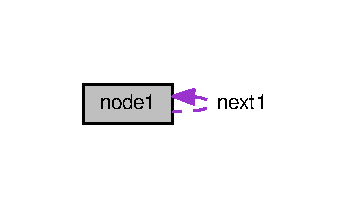
\includegraphics[width=169pt]{structnode1__coll__graph}
\end{center}
\end{figure}
\subsection*{Public Attributes}
\begin{DoxyCompactItemize}
\item 
int \hyperlink{structnode1_a3b6a50ecb2a2883e7a0a364ce108d2ad}{data1}
\item 
\hyperlink{structnode1}{node1} $\ast$ \hyperlink{structnode1_a91021c80c43acf0a49ffec9b73bf46ad}{next1}
\end{DoxyCompactItemize}


\subsection{Member Data Documentation}
\index{node1@{node1}!data1@{data1}}
\index{data1@{data1}!node1@{node1}}
\subsubsection[{\texorpdfstring{data1}{data1}}]{\setlength{\rightskip}{0pt plus 5cm}int node1\+::data1}\hypertarget{structnode1_a3b6a50ecb2a2883e7a0a364ce108d2ad}{}\label{structnode1_a3b6a50ecb2a2883e7a0a364ce108d2ad}
\index{node1@{node1}!next1@{next1}}
\index{next1@{next1}!node1@{node1}}
\subsubsection[{\texorpdfstring{next1}{next1}}]{\setlength{\rightskip}{0pt plus 5cm}{\bf node1}$\ast$ node1\+::next1}\hypertarget{structnode1_a91021c80c43acf0a49ffec9b73bf46ad}{}\label{structnode1_a91021c80c43acf0a49ffec9b73bf46ad}


The documentation for this struct was generated from the following file\+:\begin{DoxyCompactItemize}
\item 
\hyperlink{Hanoi_8cpp}{Hanoi.\+cpp}\end{DoxyCompactItemize}

\hypertarget{structnode2}{}\section{node2 Struct Reference}
\label{structnode2}\index{node2@{node2}}


Collaboration diagram for node2\+:
\nopagebreak
\begin{figure}[H]
\begin{center}
\leavevmode
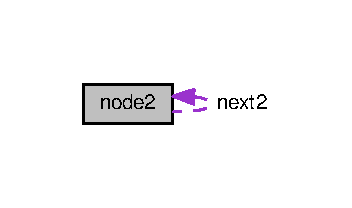
\includegraphics[width=169pt]{structnode2__coll__graph}
\end{center}
\end{figure}
\subsection*{Public Attributes}
\begin{DoxyCompactItemize}
\item 
int \hyperlink{structnode2_ac38e75c0b249b933c51d09adc1a666a0}{data2}
\item 
\hyperlink{structnode2}{node2} $\ast$ \hyperlink{structnode2_af74ee79191b380680f1546772bdd5b75}{next2}
\end{DoxyCompactItemize}


\subsection{Member Data Documentation}
\index{node2@{node2}!data2@{data2}}
\index{data2@{data2}!node2@{node2}}
\subsubsection[{\texorpdfstring{data2}{data2}}]{\setlength{\rightskip}{0pt plus 5cm}int node2\+::data2}\hypertarget{structnode2_ac38e75c0b249b933c51d09adc1a666a0}{}\label{structnode2_ac38e75c0b249b933c51d09adc1a666a0}
\index{node2@{node2}!next2@{next2}}
\index{next2@{next2}!node2@{node2}}
\subsubsection[{\texorpdfstring{next2}{next2}}]{\setlength{\rightskip}{0pt plus 5cm}{\bf node2}$\ast$ node2\+::next2}\hypertarget{structnode2_af74ee79191b380680f1546772bdd5b75}{}\label{structnode2_af74ee79191b380680f1546772bdd5b75}


The documentation for this struct was generated from the following file\+:\begin{DoxyCompactItemize}
\item 
\hyperlink{Hanoi_8cpp}{Hanoi.\+cpp}\end{DoxyCompactItemize}

\hypertarget{structnode3}{}\section{node3 Struct Reference}
\label{structnode3}\index{node3@{node3}}


Collaboration diagram for node3\+:
\nopagebreak
\begin{figure}[H]
\begin{center}
\leavevmode
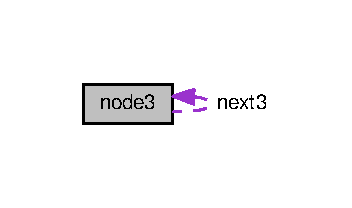
\includegraphics[width=169pt]{structnode3__coll__graph}
\end{center}
\end{figure}
\subsection*{Public Attributes}
\begin{DoxyCompactItemize}
\item 
int \hyperlink{structnode3_a6c21d03cc1ba8392be4e7fc60406a987}{data3}
\item 
\hyperlink{structnode3}{node3} $\ast$ \hyperlink{structnode3_a342e0c7f13d00bc39454b6fedaec5998}{next3}
\end{DoxyCompactItemize}


\subsection{Member Data Documentation}
\index{node3@{node3}!data3@{data3}}
\index{data3@{data3}!node3@{node3}}
\subsubsection[{\texorpdfstring{data3}{data3}}]{\setlength{\rightskip}{0pt plus 5cm}int node3\+::data3}\hypertarget{structnode3_a6c21d03cc1ba8392be4e7fc60406a987}{}\label{structnode3_a6c21d03cc1ba8392be4e7fc60406a987}
\index{node3@{node3}!next3@{next3}}
\index{next3@{next3}!node3@{node3}}
\subsubsection[{\texorpdfstring{next3}{next3}}]{\setlength{\rightskip}{0pt plus 5cm}{\bf node3}$\ast$ node3\+::next3}\hypertarget{structnode3_a342e0c7f13d00bc39454b6fedaec5998}{}\label{structnode3_a342e0c7f13d00bc39454b6fedaec5998}


The documentation for this struct was generated from the following file\+:\begin{DoxyCompactItemize}
\item 
\hyperlink{Hanoi_8cpp}{Hanoi.\+cpp}\end{DoxyCompactItemize}

\chapter{File Documentation}
\hypertarget{Hanoi_8cpp}{}\section{Hanoi.\+cpp File Reference}
\label{Hanoi_8cpp}\index{Hanoi.\+cpp@{Hanoi.\+cpp}}
{\ttfamily \#include $<$stdio.\+h$>$}\\*
{\ttfamily \#include $<$conio.\+h$>$}\\*
{\ttfamily \#include $<$iostream$>$}\\*
{\ttfamily \#include $<$math.\+h$>$}\\*
Include dependency graph for Hanoi.\+cpp\+:
\nopagebreak
\begin{figure}[H]
\begin{center}
\leavevmode
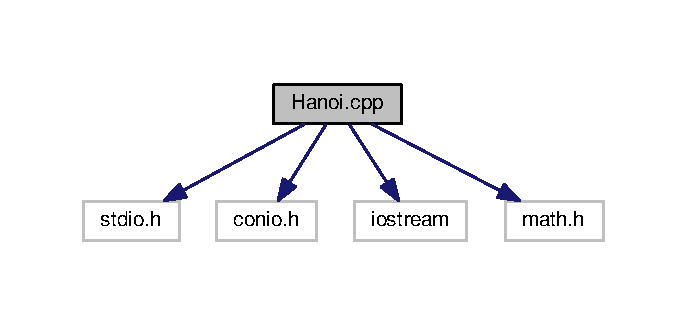
\includegraphics[width=330pt]{Hanoi_8cpp__incl}
\end{center}
\end{figure}
\subsection*{Classes}
\begin{DoxyCompactItemize}
\item 
struct \hyperlink{structnode1}{node1}
\item 
struct \hyperlink{structnode2}{node2}
\item 
struct \hyperlink{structnode3}{node3}
\end{DoxyCompactItemize}
\subsection*{Functions}
\begin{DoxyCompactItemize}
\item 
void \hyperlink{Hanoi_8cpp_a1fce6374e1ef4cb024c6b01e30a43f68}{push1} (int data)
\item 
int \hyperlink{Hanoi_8cpp_af58e39ad89f8cfa75b98b1257bcf36a0}{pop1} ()
\item 
void \hyperlink{Hanoi_8cpp_a767b7e679d8c5d22a580db03990ea12f}{push2} (int data)
\item 
int \hyperlink{Hanoi_8cpp_a882f158fc965ebb96b194da3ae94521f}{pop2} ()
\item 
void \hyperlink{Hanoi_8cpp_a9ccc836d1bbc190a76294396ff8f666e}{push3} (int data)
\item 
int \hyperlink{Hanoi_8cpp_a2931e808c631764310a317aef61576b6}{pop3} ()
\item 
int \hyperlink{Hanoi_8cpp_a291e39ca05e6be6177ed666fad1b6648}{top\+\_\+of\+\_\+stack} ()
\item 
void \hyperlink{Hanoi_8cpp_af4b6db54ef371626a3d23da2636a4fa0}{display1} ()
\item 
void \hyperlink{Hanoi_8cpp_a91cdf55e49e2c33dd11a85a178a82409}{display2} ()
\item 
void \hyperlink{Hanoi_8cpp_a5ae730bf155322af402f2f4b2dfcd54d}{display3} ()
\item 
void \hyperlink{Hanoi_8cpp_a4932224a815c7bc7f923a709867b60c8}{toh} (int n)
\item 
int \hyperlink{Hanoi_8cpp_ae66f6b31b5ad750f1fe042a706a4e3d4}{main} ()
\end{DoxyCompactItemize}
\subsection*{Variables}
\begin{DoxyCompactItemize}
\item 
struct \hyperlink{structnode1}{node1} $\ast$ \hyperlink{Hanoi_8cpp_a4ee7dfa04c6334adbe54a10633e0a836}{top1} = N\+U\+LL
\item 
struct \hyperlink{structnode1}{node1} $\ast$ \hyperlink{Hanoi_8cpp_a32652b709ed43d8af2941c59ec0a1794}{p1} = N\+U\+LL
\item 
struct \hyperlink{structnode1}{node1} $\ast$ \hyperlink{Hanoi_8cpp_af2631d988504474b2e0882737b7bb156}{np1} = N\+U\+LL
\item 
struct \hyperlink{structnode2}{node2} $\ast$ \hyperlink{Hanoi_8cpp_aff896aceb3f9a2daf3f46595fa7a2d52}{top2} = N\+U\+LL
\item 
struct \hyperlink{structnode2}{node2} $\ast$ \hyperlink{Hanoi_8cpp_a638d198cd87dbff473994ab55d4e6ddb}{p2} = N\+U\+LL
\item 
struct \hyperlink{structnode2}{node2} $\ast$ \hyperlink{Hanoi_8cpp_a10d1d4439d1217e35ff279db8b646cbe}{np2} = N\+U\+LL
\item 
struct \hyperlink{structnode3}{node3} $\ast$ \hyperlink{Hanoi_8cpp_ab7494ef86b6ca5727eec7a533472c462}{top3} = N\+U\+LL
\item 
struct \hyperlink{structnode3}{node3} $\ast$ \hyperlink{Hanoi_8cpp_abb53896a33e6ac94f4a8011cc32b34c1}{p3} = N\+U\+LL
\item 
struct \hyperlink{structnode3}{node3} $\ast$ \hyperlink{Hanoi_8cpp_a0c696bf1e4e27bbde20f5e8b5dde34fe}{np3} = N\+U\+LL
\end{DoxyCompactItemize}


\subsection{Function Documentation}
\index{Hanoi.\+cpp@{Hanoi.\+cpp}!display1@{display1}}
\index{display1@{display1}!Hanoi.\+cpp@{Hanoi.\+cpp}}
\subsubsection[{\texorpdfstring{display1()}{display1()}}]{\setlength{\rightskip}{0pt plus 5cm}void display1 (
\begin{DoxyParamCaption}
{}
\end{DoxyParamCaption}
)}\hypertarget{Hanoi_8cpp_af4b6db54ef371626a3d23da2636a4fa0}{}\label{Hanoi_8cpp_af4b6db54ef371626a3d23da2636a4fa0}

\begin{DoxyCode}
130 \{
131     cout<<endl;
132     \hyperlink{structnode1}{node1} *\hyperlink{Hanoi_8cpp_a32652b709ed43d8af2941c59ec0a1794}{p1};
133     p1 = \hyperlink{Hanoi_8cpp_a4ee7dfa04c6334adbe54a10633e0a836}{top1};
134     cout<<\textcolor{stringliteral}{"Tower1-> "}<<\textcolor{stringliteral}{"\(\backslash\)t"};
135     \textcolor{keywordflow}{while} (p1 != NULL)
136     \{
137         cout<<p1->\hyperlink{structnode1_a3b6a50ecb2a2883e7a0a364ce108d2ad}{data1}<<\textcolor{stringliteral}{"\(\backslash\)t"};
138         p1 = p1->\hyperlink{structnode1_a91021c80c43acf0a49ffec9b73bf46ad}{next1};
139     \}
140     cout<<endl;
141 \}
\end{DoxyCode}
\index{Hanoi.\+cpp@{Hanoi.\+cpp}!display2@{display2}}
\index{display2@{display2}!Hanoi.\+cpp@{Hanoi.\+cpp}}
\subsubsection[{\texorpdfstring{display2()}{display2()}}]{\setlength{\rightskip}{0pt plus 5cm}void display2 (
\begin{DoxyParamCaption}
{}
\end{DoxyParamCaption}
)}\hypertarget{Hanoi_8cpp_a91cdf55e49e2c33dd11a85a178a82409}{}\label{Hanoi_8cpp_a91cdf55e49e2c33dd11a85a178a82409}

\begin{DoxyCode}
143 \{
144     \hyperlink{structnode2}{node2} *\hyperlink{Hanoi_8cpp_a638d198cd87dbff473994ab55d4e6ddb}{p2};
145     p2 = \hyperlink{Hanoi_8cpp_aff896aceb3f9a2daf3f46595fa7a2d52}{top2};
146     cout<<\textcolor{stringliteral}{"Tower2-> "}<<\textcolor{stringliteral}{"\(\backslash\)t"};
147     \textcolor{keywordflow}{while} (p2 != NULL)
148     \{
149         cout<<p2->\hyperlink{structnode2_ac38e75c0b249b933c51d09adc1a666a0}{data2}<<\textcolor{stringliteral}{"\(\backslash\)t"};
150         p2 = p2->\hyperlink{structnode2_af74ee79191b380680f1546772bdd5b75}{next2};
151     \}
152     cout<<endl;
153 \}
\end{DoxyCode}
\index{Hanoi.\+cpp@{Hanoi.\+cpp}!display3@{display3}}
\index{display3@{display3}!Hanoi.\+cpp@{Hanoi.\+cpp}}
\subsubsection[{\texorpdfstring{display3()}{display3()}}]{\setlength{\rightskip}{0pt plus 5cm}void display3 (
\begin{DoxyParamCaption}
{}
\end{DoxyParamCaption}
)}\hypertarget{Hanoi_8cpp_a5ae730bf155322af402f2f4b2dfcd54d}{}\label{Hanoi_8cpp_a5ae730bf155322af402f2f4b2dfcd54d}

\begin{DoxyCode}
155 \{
156     \hyperlink{structnode3}{node3} *\hyperlink{Hanoi_8cpp_abb53896a33e6ac94f4a8011cc32b34c1}{p3};
157     p3 = \hyperlink{Hanoi_8cpp_ab7494ef86b6ca5727eec7a533472c462}{top3};
158     cout<<\textcolor{stringliteral}{"Tower3-> "}<<\textcolor{stringliteral}{"\(\backslash\)t"};
159     \textcolor{keywordflow}{while} (p3 != NULL)
160     \{
161         cout<<p3->\hyperlink{structnode3_a6c21d03cc1ba8392be4e7fc60406a987}{data3}<<\textcolor{stringliteral}{"\(\backslash\)t"};
162         p3 = p3->\hyperlink{structnode3_a342e0c7f13d00bc39454b6fedaec5998}{next3};
163     \}
164     cout<<endl;
165     cout<<endl;
166 \}
\end{DoxyCode}
\index{Hanoi.\+cpp@{Hanoi.\+cpp}!main@{main}}
\index{main@{main}!Hanoi.\+cpp@{Hanoi.\+cpp}}
\subsubsection[{\texorpdfstring{main()}{main()}}]{\setlength{\rightskip}{0pt plus 5cm}int main (
\begin{DoxyParamCaption}
{}
\end{DoxyParamCaption}
)}\hypertarget{Hanoi_8cpp_ae66f6b31b5ad750f1fe042a706a4e3d4}{}\label{Hanoi_8cpp_ae66f6b31b5ad750f1fe042a706a4e3d4}

\begin{DoxyCode}
266 \{
267     \textcolor{keywordtype}{int} n, i;
268     cout<<\textcolor{stringliteral}{"enter the number of disks\(\backslash\)n"};
269     cin>>n;
270     \textcolor{keywordflow}{for} (i = n; i >= 1; i--)
271     \{
272         \hyperlink{Hanoi_8cpp_a1fce6374e1ef4cb024c6b01e30a43f68}{push1}(i);
273     \} 
274     \hyperlink{Hanoi_8cpp_a4932224a815c7bc7f923a709867b60c8}{toh}(n);
275     getch();
276 \}
\end{DoxyCode}


Here is the call graph for this function\+:
\nopagebreak
\begin{figure}[H]
\begin{center}
\leavevmode
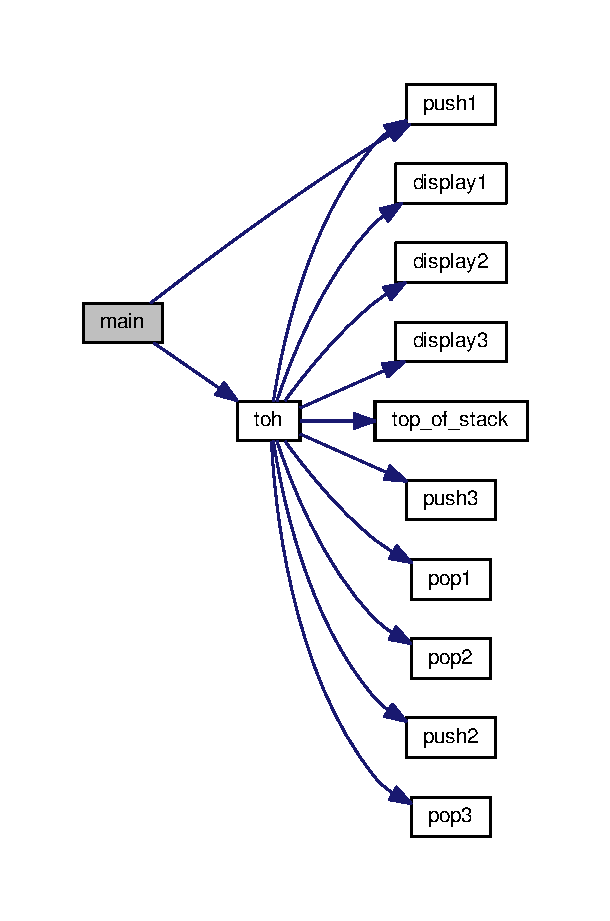
\includegraphics[width=293pt]{Hanoi_8cpp_ae66f6b31b5ad750f1fe042a706a4e3d4_cgraph}
\end{center}
\end{figure}


\index{Hanoi.\+cpp@{Hanoi.\+cpp}!pop1@{pop1}}
\index{pop1@{pop1}!Hanoi.\+cpp@{Hanoi.\+cpp}}
\subsubsection[{\texorpdfstring{pop1()}{pop1()}}]{\setlength{\rightskip}{0pt plus 5cm}int pop1 (
\begin{DoxyParamCaption}
{}
\end{DoxyParamCaption}
)}\hypertarget{Hanoi_8cpp_af58e39ad89f8cfa75b98b1257bcf36a0}{}\label{Hanoi_8cpp_af58e39ad89f8cfa75b98b1257bcf36a0}

\begin{DoxyCode}
40 \{
41     \textcolor{keywordtype}{int} b = 999;
42     \textcolor{keywordflow}{if} (\hyperlink{Hanoi_8cpp_a4ee7dfa04c6334adbe54a10633e0a836}{top1} == NULL)
43     \{
44         \textcolor{keywordflow}{return} b;
45     \}
46     \textcolor{keywordflow}{else}
47     \{
48         \hyperlink{Hanoi_8cpp_a32652b709ed43d8af2941c59ec0a1794}{p1} = \hyperlink{Hanoi_8cpp_a4ee7dfa04c6334adbe54a10633e0a836}{top1};
49         \hyperlink{Hanoi_8cpp_a4ee7dfa04c6334adbe54a10633e0a836}{top1} = \hyperlink{Hanoi_8cpp_a4ee7dfa04c6334adbe54a10633e0a836}{top1}->\hyperlink{structnode1_a91021c80c43acf0a49ffec9b73bf46ad}{next1};
50         \textcolor{keywordflow}{return}(\hyperlink{Hanoi_8cpp_a32652b709ed43d8af2941c59ec0a1794}{p1}->\hyperlink{structnode1_a3b6a50ecb2a2883e7a0a364ce108d2ad}{data1});
51         \textcolor{keyword}{delete}(\hyperlink{Hanoi_8cpp_a32652b709ed43d8af2941c59ec0a1794}{p1});
52     \}
53 \}
\end{DoxyCode}
\index{Hanoi.\+cpp@{Hanoi.\+cpp}!pop2@{pop2}}
\index{pop2@{pop2}!Hanoi.\+cpp@{Hanoi.\+cpp}}
\subsubsection[{\texorpdfstring{pop2()}{pop2()}}]{\setlength{\rightskip}{0pt plus 5cm}int pop2 (
\begin{DoxyParamCaption}
{}
\end{DoxyParamCaption}
)}\hypertarget{Hanoi_8cpp_a882f158fc965ebb96b194da3ae94521f}{}\label{Hanoi_8cpp_a882f158fc965ebb96b194da3ae94521f}

\begin{DoxyCode}
70 \{
71     \textcolor{keywordtype}{int} b = 999;
72     \textcolor{keywordflow}{if} (\hyperlink{Hanoi_8cpp_aff896aceb3f9a2daf3f46595fa7a2d52}{top2} == NULL)
73     \{
74         \textcolor{keywordflow}{return} b;
75     \}
76     \textcolor{keywordflow}{else}
77     \{
78         \hyperlink{Hanoi_8cpp_a638d198cd87dbff473994ab55d4e6ddb}{p2} = \hyperlink{Hanoi_8cpp_aff896aceb3f9a2daf3f46595fa7a2d52}{top2};
79         \hyperlink{Hanoi_8cpp_aff896aceb3f9a2daf3f46595fa7a2d52}{top2} = \hyperlink{Hanoi_8cpp_aff896aceb3f9a2daf3f46595fa7a2d52}{top2}->\hyperlink{structnode2_af74ee79191b380680f1546772bdd5b75}{next2};
80         \textcolor{keywordflow}{return}(\hyperlink{Hanoi_8cpp_a638d198cd87dbff473994ab55d4e6ddb}{p2}->\hyperlink{structnode2_ac38e75c0b249b933c51d09adc1a666a0}{data2});
81         \textcolor{keyword}{delete}(\hyperlink{Hanoi_8cpp_a638d198cd87dbff473994ab55d4e6ddb}{p2});
82     \}
83 \}
\end{DoxyCode}
\index{Hanoi.\+cpp@{Hanoi.\+cpp}!pop3@{pop3}}
\index{pop3@{pop3}!Hanoi.\+cpp@{Hanoi.\+cpp}}
\subsubsection[{\texorpdfstring{pop3()}{pop3()}}]{\setlength{\rightskip}{0pt plus 5cm}int pop3 (
\begin{DoxyParamCaption}
{}
\end{DoxyParamCaption}
)}\hypertarget{Hanoi_8cpp_a2931e808c631764310a317aef61576b6}{}\label{Hanoi_8cpp_a2931e808c631764310a317aef61576b6}

\begin{DoxyCode}
100 \{
101     \textcolor{keywordtype}{int} b = 999;
102     \textcolor{keywordflow}{if} (\hyperlink{Hanoi_8cpp_ab7494ef86b6ca5727eec7a533472c462}{top3} == NULL)
103     \{
104         \textcolor{keywordflow}{return} b;
105     \}
106     \textcolor{keywordflow}{else}
107     \{
108         \hyperlink{Hanoi_8cpp_abb53896a33e6ac94f4a8011cc32b34c1}{p3} = \hyperlink{Hanoi_8cpp_ab7494ef86b6ca5727eec7a533472c462}{top3};
109         \hyperlink{Hanoi_8cpp_ab7494ef86b6ca5727eec7a533472c462}{top3} = \hyperlink{Hanoi_8cpp_ab7494ef86b6ca5727eec7a533472c462}{top3}->\hyperlink{structnode3_a342e0c7f13d00bc39454b6fedaec5998}{next3};
110         \textcolor{keywordflow}{return}(\hyperlink{Hanoi_8cpp_abb53896a33e6ac94f4a8011cc32b34c1}{p3}->\hyperlink{structnode3_a6c21d03cc1ba8392be4e7fc60406a987}{data3});
111         \textcolor{keyword}{delete}(\hyperlink{Hanoi_8cpp_abb53896a33e6ac94f4a8011cc32b34c1}{p3});
112     \}
113 \}
\end{DoxyCode}
\index{Hanoi.\+cpp@{Hanoi.\+cpp}!push1@{push1}}
\index{push1@{push1}!Hanoi.\+cpp@{Hanoi.\+cpp}}
\subsubsection[{\texorpdfstring{push1(int data)}{push1(int data)}}]{\setlength{\rightskip}{0pt plus 5cm}void push1 (
\begin{DoxyParamCaption}
\item[{int}]{data}
\end{DoxyParamCaption}
)}\hypertarget{Hanoi_8cpp_a1fce6374e1ef4cb024c6b01e30a43f68}{}\label{Hanoi_8cpp_a1fce6374e1ef4cb024c6b01e30a43f68}

\begin{DoxyCode}
25 \{
26     \hyperlink{Hanoi_8cpp_af2631d988504474b2e0882737b7bb156}{np1} = \textcolor{keyword}{new} \hyperlink{structnode1}{node1};
27     \hyperlink{Hanoi_8cpp_af2631d988504474b2e0882737b7bb156}{np1}->\hyperlink{structnode1_a3b6a50ecb2a2883e7a0a364ce108d2ad}{data1} = data;
28     \hyperlink{Hanoi_8cpp_af2631d988504474b2e0882737b7bb156}{np1}->\hyperlink{structnode1_a91021c80c43acf0a49ffec9b73bf46ad}{next1} = NULL;
29     \textcolor{keywordflow}{if} (\hyperlink{Hanoi_8cpp_a4ee7dfa04c6334adbe54a10633e0a836}{top1} == NULL)
30     \{
31         \hyperlink{Hanoi_8cpp_a4ee7dfa04c6334adbe54a10633e0a836}{top1} = \hyperlink{Hanoi_8cpp_af2631d988504474b2e0882737b7bb156}{np1};
32     \}
33     \textcolor{keywordflow}{else}
34     \{
35         \hyperlink{Hanoi_8cpp_af2631d988504474b2e0882737b7bb156}{np1}->\hyperlink{structnode1_a91021c80c43acf0a49ffec9b73bf46ad}{next1} = \hyperlink{Hanoi_8cpp_a4ee7dfa04c6334adbe54a10633e0a836}{top1};
36         \hyperlink{Hanoi_8cpp_a4ee7dfa04c6334adbe54a10633e0a836}{top1} = \hyperlink{Hanoi_8cpp_af2631d988504474b2e0882737b7bb156}{np1};
37     \}
38 \}
\end{DoxyCode}
\index{Hanoi.\+cpp@{Hanoi.\+cpp}!push2@{push2}}
\index{push2@{push2}!Hanoi.\+cpp@{Hanoi.\+cpp}}
\subsubsection[{\texorpdfstring{push2(int data)}{push2(int data)}}]{\setlength{\rightskip}{0pt plus 5cm}void push2 (
\begin{DoxyParamCaption}
\item[{int}]{data}
\end{DoxyParamCaption}
)}\hypertarget{Hanoi_8cpp_a767b7e679d8c5d22a580db03990ea12f}{}\label{Hanoi_8cpp_a767b7e679d8c5d22a580db03990ea12f}

\begin{DoxyCode}
55 \{
56     \hyperlink{Hanoi_8cpp_a10d1d4439d1217e35ff279db8b646cbe}{np2} = \textcolor{keyword}{new} \hyperlink{structnode2}{node2};
57     \hyperlink{Hanoi_8cpp_a10d1d4439d1217e35ff279db8b646cbe}{np2}->\hyperlink{structnode2_ac38e75c0b249b933c51d09adc1a666a0}{data2} = data;
58     \hyperlink{Hanoi_8cpp_a10d1d4439d1217e35ff279db8b646cbe}{np2}->\hyperlink{structnode2_af74ee79191b380680f1546772bdd5b75}{next2} = NULL;
59     \textcolor{keywordflow}{if} (\hyperlink{Hanoi_8cpp_aff896aceb3f9a2daf3f46595fa7a2d52}{top2} == NULL)
60     \{
61         \hyperlink{Hanoi_8cpp_aff896aceb3f9a2daf3f46595fa7a2d52}{top2} = \hyperlink{Hanoi_8cpp_a10d1d4439d1217e35ff279db8b646cbe}{np2};
62     \}
63     \textcolor{keywordflow}{else}
64     \{
65         \hyperlink{Hanoi_8cpp_a10d1d4439d1217e35ff279db8b646cbe}{np2}->\hyperlink{structnode2_af74ee79191b380680f1546772bdd5b75}{next2} = \hyperlink{Hanoi_8cpp_aff896aceb3f9a2daf3f46595fa7a2d52}{top2};
66         \hyperlink{Hanoi_8cpp_aff896aceb3f9a2daf3f46595fa7a2d52}{top2} = \hyperlink{Hanoi_8cpp_a10d1d4439d1217e35ff279db8b646cbe}{np2};
67     \}
68 \}
\end{DoxyCode}
\index{Hanoi.\+cpp@{Hanoi.\+cpp}!push3@{push3}}
\index{push3@{push3}!Hanoi.\+cpp@{Hanoi.\+cpp}}
\subsubsection[{\texorpdfstring{push3(int data)}{push3(int data)}}]{\setlength{\rightskip}{0pt plus 5cm}void push3 (
\begin{DoxyParamCaption}
\item[{int}]{data}
\end{DoxyParamCaption}
)}\hypertarget{Hanoi_8cpp_a9ccc836d1bbc190a76294396ff8f666e}{}\label{Hanoi_8cpp_a9ccc836d1bbc190a76294396ff8f666e}

\begin{DoxyCode}
85 \{
86     \hyperlink{Hanoi_8cpp_a0c696bf1e4e27bbde20f5e8b5dde34fe}{np3} = \textcolor{keyword}{new} \hyperlink{structnode3}{node3};
87     \hyperlink{Hanoi_8cpp_a0c696bf1e4e27bbde20f5e8b5dde34fe}{np3}->\hyperlink{structnode3_a6c21d03cc1ba8392be4e7fc60406a987}{data3} = data;
88     \hyperlink{Hanoi_8cpp_a0c696bf1e4e27bbde20f5e8b5dde34fe}{np3}->\hyperlink{structnode3_a342e0c7f13d00bc39454b6fedaec5998}{next3} = NULL;
89     \textcolor{keywordflow}{if} (\hyperlink{Hanoi_8cpp_ab7494ef86b6ca5727eec7a533472c462}{top3} == NULL)
90     \{
91         \hyperlink{Hanoi_8cpp_ab7494ef86b6ca5727eec7a533472c462}{top3} = \hyperlink{Hanoi_8cpp_a0c696bf1e4e27bbde20f5e8b5dde34fe}{np3};
92     \}
93     \textcolor{keywordflow}{else}
94     \{
95         \hyperlink{Hanoi_8cpp_a0c696bf1e4e27bbde20f5e8b5dde34fe}{np3}->\hyperlink{structnode3_a342e0c7f13d00bc39454b6fedaec5998}{next3} = \hyperlink{Hanoi_8cpp_ab7494ef86b6ca5727eec7a533472c462}{top3};
96         \hyperlink{Hanoi_8cpp_ab7494ef86b6ca5727eec7a533472c462}{top3} = \hyperlink{Hanoi_8cpp_a0c696bf1e4e27bbde20f5e8b5dde34fe}{np3};
97     \}
98 \}
\end{DoxyCode}
\index{Hanoi.\+cpp@{Hanoi.\+cpp}!toh@{toh}}
\index{toh@{toh}!Hanoi.\+cpp@{Hanoi.\+cpp}}
\subsubsection[{\texorpdfstring{toh(int n)}{toh(int n)}}]{\setlength{\rightskip}{0pt plus 5cm}void toh (
\begin{DoxyParamCaption}
\item[{int}]{n}
\end{DoxyParamCaption}
)}\hypertarget{Hanoi_8cpp_a4932224a815c7bc7f923a709867b60c8}{}\label{Hanoi_8cpp_a4932224a815c7bc7f923a709867b60c8}

\begin{DoxyCode}
168 \{
169     \textcolor{keywordtype}{int} i, x, a, b;
170     \textcolor{keywordflow}{for} (i = 0; i < (pow(2,n)); i++)
171     \{
172         \hyperlink{Hanoi_8cpp_af4b6db54ef371626a3d23da2636a4fa0}{display1}();
173         \hyperlink{Hanoi_8cpp_a91cdf55e49e2c33dd11a85a178a82409}{display2}();
174         \hyperlink{Hanoi_8cpp_a5ae730bf155322af402f2f4b2dfcd54d}{display3}();
175         x = \hyperlink{Hanoi_8cpp_a291e39ca05e6be6177ed666fad1b6648}{top\_of\_stack}();
176         \textcolor{keywordflow}{if} (i % 2 == 0)
177         \{
178             \textcolor{keywordflow}{if} (x == 1)
179             \{
180                 \hyperlink{Hanoi_8cpp_a9ccc836d1bbc190a76294396ff8f666e}{push3}(\hyperlink{Hanoi_8cpp_af58e39ad89f8cfa75b98b1257bcf36a0}{pop1}());
181             \}
182             \textcolor{keywordflow}{else} \textcolor{keywordflow}{if} (x == 2)
183             \{
184                 \hyperlink{Hanoi_8cpp_a1fce6374e1ef4cb024c6b01e30a43f68}{push1}(\hyperlink{Hanoi_8cpp_a882f158fc965ebb96b194da3ae94521f}{pop2}());
185             \}
186             \textcolor{keywordflow}{else} \textcolor{keywordflow}{if} (x == 3)
187             \{
188                 \hyperlink{Hanoi_8cpp_a767b7e679d8c5d22a580db03990ea12f}{push2}(\hyperlink{Hanoi_8cpp_a2931e808c631764310a317aef61576b6}{pop3}());
189             \}
190         \}
191         \textcolor{keywordflow}{else}
192         \{
193             \textcolor{keywordflow}{if} (x == 1)
194             \{
195                 a = \hyperlink{Hanoi_8cpp_a882f158fc965ebb96b194da3ae94521f}{pop2}();
196                 b = \hyperlink{Hanoi_8cpp_a2931e808c631764310a317aef61576b6}{pop3}();
197                 \textcolor{keywordflow}{if} (a < b && b != 999)
198                 \{
199                     \hyperlink{Hanoi_8cpp_a9ccc836d1bbc190a76294396ff8f666e}{push3}(b);
200                     \hyperlink{Hanoi_8cpp_a9ccc836d1bbc190a76294396ff8f666e}{push3}(a);
201                 \}
202                 \textcolor{keywordflow}{else} \textcolor{keywordflow}{if} (a > b && a != 999)
203                 \{
204                     \hyperlink{Hanoi_8cpp_a767b7e679d8c5d22a580db03990ea12f}{push2}(a);
205                     \hyperlink{Hanoi_8cpp_a767b7e679d8c5d22a580db03990ea12f}{push2}(b);
206                 \}
207                 \textcolor{keywordflow}{else} \textcolor{keywordflow}{if} (b == 999)
208                 \{
209                     \hyperlink{Hanoi_8cpp_a9ccc836d1bbc190a76294396ff8f666e}{push3}(a);
210                 \}
211                 \textcolor{keywordflow}{else} \textcolor{keywordflow}{if} (a == 999)
212                 \{
213                     \hyperlink{Hanoi_8cpp_a767b7e679d8c5d22a580db03990ea12f}{push2}(b);
214                 \}
215             \}
216             \textcolor{keywordflow}{else} \textcolor{keywordflow}{if} (x == 2)
217             \{
218                 a = \hyperlink{Hanoi_8cpp_af58e39ad89f8cfa75b98b1257bcf36a0}{pop1}();
219                 b = \hyperlink{Hanoi_8cpp_a2931e808c631764310a317aef61576b6}{pop3}();
220                 \textcolor{keywordflow}{if} (a < b && b != 999)
221                 \{
222                     \hyperlink{Hanoi_8cpp_a9ccc836d1bbc190a76294396ff8f666e}{push3}(b);
223                     \hyperlink{Hanoi_8cpp_a9ccc836d1bbc190a76294396ff8f666e}{push3}(a);
224                 \}
225                 \textcolor{keywordflow}{else} \textcolor{keywordflow}{if} (a > b && a != 999)
226                 \{
227                     \hyperlink{Hanoi_8cpp_a1fce6374e1ef4cb024c6b01e30a43f68}{push1}(a);
228                     \hyperlink{Hanoi_8cpp_a1fce6374e1ef4cb024c6b01e30a43f68}{push1}(b);
229                 \}
230                 \textcolor{keywordflow}{else} \textcolor{keywordflow}{if} (b == 999)
231                 \{
232                     \hyperlink{Hanoi_8cpp_a9ccc836d1bbc190a76294396ff8f666e}{push3}(a);
233                 \}
234                 \textcolor{keywordflow}{else} \textcolor{keywordflow}{if} (a == 999)
235                 \{
236                     \hyperlink{Hanoi_8cpp_a1fce6374e1ef4cb024c6b01e30a43f68}{push1}(b);
237                 \}
238             \}
239             \textcolor{keywordflow}{else} \textcolor{keywordflow}{if} (x == 3)
240             \{
241                 a = \hyperlink{Hanoi_8cpp_af58e39ad89f8cfa75b98b1257bcf36a0}{pop1}();
242                 b = \hyperlink{Hanoi_8cpp_a882f158fc965ebb96b194da3ae94521f}{pop2}();
243                 \textcolor{keywordflow}{if} (a < b && b != 999)
244                 \{
245                     \hyperlink{Hanoi_8cpp_a767b7e679d8c5d22a580db03990ea12f}{push2}(b);
246                     \hyperlink{Hanoi_8cpp_a767b7e679d8c5d22a580db03990ea12f}{push2}(a);
247                 \}
248                 \textcolor{keywordflow}{else} \textcolor{keywordflow}{if} (a > b && a != 999)
249                 \{
250                     \hyperlink{Hanoi_8cpp_a1fce6374e1ef4cb024c6b01e30a43f68}{push1}(a);
251                     \hyperlink{Hanoi_8cpp_a1fce6374e1ef4cb024c6b01e30a43f68}{push1}(b);
252                 \}
253                 \textcolor{keywordflow}{else} \textcolor{keywordflow}{if} (b == 999)
254                 \{
255                     \hyperlink{Hanoi_8cpp_a767b7e679d8c5d22a580db03990ea12f}{push2}(a);
256                 \}
257                 \textcolor{keywordflow}{else} \textcolor{keywordflow}{if} (a == 999)
258                 \{
259                     \hyperlink{Hanoi_8cpp_a1fce6374e1ef4cb024c6b01e30a43f68}{push1}(b);
260                 \}
261             \}
262         \}
263     \}
264 \}
\end{DoxyCode}


Here is the call graph for this function\+:
\nopagebreak
\begin{figure}[H]
\begin{center}
\leavevmode
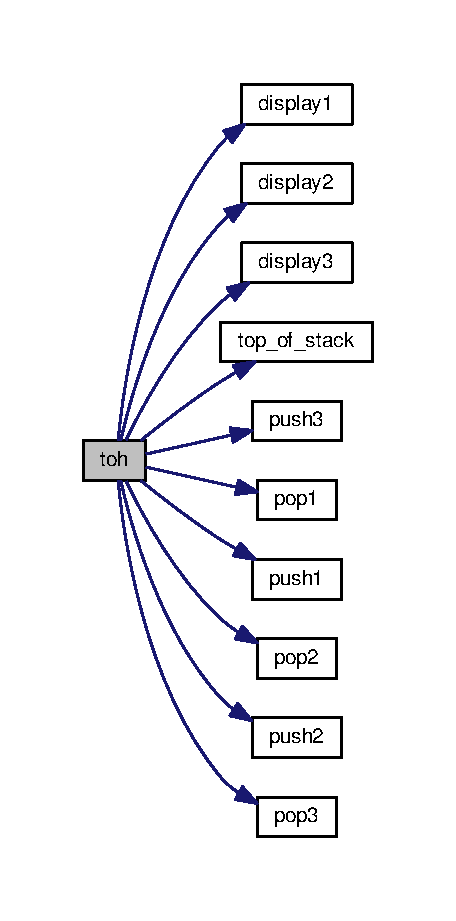
\includegraphics[width=219pt]{Hanoi_8cpp_a4932224a815c7bc7f923a709867b60c8_cgraph}
\end{center}
\end{figure}


\index{Hanoi.\+cpp@{Hanoi.\+cpp}!top\+\_\+of\+\_\+stack@{top\+\_\+of\+\_\+stack}}
\index{top\+\_\+of\+\_\+stack@{top\+\_\+of\+\_\+stack}!Hanoi.\+cpp@{Hanoi.\+cpp}}
\subsubsection[{\texorpdfstring{top\+\_\+of\+\_\+stack()}{top_of_stack()}}]{\setlength{\rightskip}{0pt plus 5cm}int top\+\_\+of\+\_\+stack (
\begin{DoxyParamCaption}
{}
\end{DoxyParamCaption}
)}\hypertarget{Hanoi_8cpp_a291e39ca05e6be6177ed666fad1b6648}{}\label{Hanoi_8cpp_a291e39ca05e6be6177ed666fad1b6648}

\begin{DoxyCode}
115 \{
116     \textcolor{keywordflow}{if} (\hyperlink{Hanoi_8cpp_a4ee7dfa04c6334adbe54a10633e0a836}{top1} != NULL && \hyperlink{Hanoi_8cpp_a4ee7dfa04c6334adbe54a10633e0a836}{top1}->\hyperlink{structnode1_a3b6a50ecb2a2883e7a0a364ce108d2ad}{data1} == 1 )
117     \{
118         \textcolor{keywordflow}{return} 1;
119     \}
120     \textcolor{keywordflow}{else} \textcolor{keywordflow}{if} (\hyperlink{Hanoi_8cpp_aff896aceb3f9a2daf3f46595fa7a2d52}{top2} != NULL && \hyperlink{Hanoi_8cpp_aff896aceb3f9a2daf3f46595fa7a2d52}{top2}->\hyperlink{structnode2_ac38e75c0b249b933c51d09adc1a666a0}{data2} == 1)
121     \{
122         \textcolor{keywordflow}{return} 2;
123     \}
124     \textcolor{keywordflow}{else} \textcolor{keywordflow}{if} (\hyperlink{Hanoi_8cpp_ab7494ef86b6ca5727eec7a533472c462}{top3} != NULL && \hyperlink{Hanoi_8cpp_ab7494ef86b6ca5727eec7a533472c462}{top3}->\hyperlink{structnode3_a6c21d03cc1ba8392be4e7fc60406a987}{data3} == 1)
125     \{
126         \textcolor{keywordflow}{return} 3;
127     \}
128 \}
\end{DoxyCode}


\subsection{Variable Documentation}
\index{Hanoi.\+cpp@{Hanoi.\+cpp}!np1@{np1}}
\index{np1@{np1}!Hanoi.\+cpp@{Hanoi.\+cpp}}
\subsubsection[{\texorpdfstring{np1}{np1}}]{\setlength{\rightskip}{0pt plus 5cm}struct {\bf node1} $\ast$ np1 = N\+U\+LL}\hypertarget{Hanoi_8cpp_af2631d988504474b2e0882737b7bb156}{}\label{Hanoi_8cpp_af2631d988504474b2e0882737b7bb156}
\index{Hanoi.\+cpp@{Hanoi.\+cpp}!np2@{np2}}
\index{np2@{np2}!Hanoi.\+cpp@{Hanoi.\+cpp}}
\subsubsection[{\texorpdfstring{np2}{np2}}]{\setlength{\rightskip}{0pt plus 5cm}struct {\bf node2} $\ast$ np2 = N\+U\+LL}\hypertarget{Hanoi_8cpp_a10d1d4439d1217e35ff279db8b646cbe}{}\label{Hanoi_8cpp_a10d1d4439d1217e35ff279db8b646cbe}
\index{Hanoi.\+cpp@{Hanoi.\+cpp}!np3@{np3}}
\index{np3@{np3}!Hanoi.\+cpp@{Hanoi.\+cpp}}
\subsubsection[{\texorpdfstring{np3}{np3}}]{\setlength{\rightskip}{0pt plus 5cm}struct {\bf node3} $\ast$ np3 = N\+U\+LL}\hypertarget{Hanoi_8cpp_a0c696bf1e4e27bbde20f5e8b5dde34fe}{}\label{Hanoi_8cpp_a0c696bf1e4e27bbde20f5e8b5dde34fe}
\index{Hanoi.\+cpp@{Hanoi.\+cpp}!p1@{p1}}
\index{p1@{p1}!Hanoi.\+cpp@{Hanoi.\+cpp}}
\subsubsection[{\texorpdfstring{p1}{p1}}]{\setlength{\rightskip}{0pt plus 5cm}struct {\bf node1} $\ast$ p1 = N\+U\+LL}\hypertarget{Hanoi_8cpp_a32652b709ed43d8af2941c59ec0a1794}{}\label{Hanoi_8cpp_a32652b709ed43d8af2941c59ec0a1794}
\index{Hanoi.\+cpp@{Hanoi.\+cpp}!p2@{p2}}
\index{p2@{p2}!Hanoi.\+cpp@{Hanoi.\+cpp}}
\subsubsection[{\texorpdfstring{p2}{p2}}]{\setlength{\rightskip}{0pt plus 5cm}struct {\bf node2} $\ast$ p2 = N\+U\+LL}\hypertarget{Hanoi_8cpp_a638d198cd87dbff473994ab55d4e6ddb}{}\label{Hanoi_8cpp_a638d198cd87dbff473994ab55d4e6ddb}
\index{Hanoi.\+cpp@{Hanoi.\+cpp}!p3@{p3}}
\index{p3@{p3}!Hanoi.\+cpp@{Hanoi.\+cpp}}
\subsubsection[{\texorpdfstring{p3}{p3}}]{\setlength{\rightskip}{0pt plus 5cm}struct {\bf node3} $\ast$ p3 = N\+U\+LL}\hypertarget{Hanoi_8cpp_abb53896a33e6ac94f4a8011cc32b34c1}{}\label{Hanoi_8cpp_abb53896a33e6ac94f4a8011cc32b34c1}
\index{Hanoi.\+cpp@{Hanoi.\+cpp}!top1@{top1}}
\index{top1@{top1}!Hanoi.\+cpp@{Hanoi.\+cpp}}
\subsubsection[{\texorpdfstring{top1}{top1}}]{\setlength{\rightskip}{0pt plus 5cm}struct {\bf node1}$\ast$ top1 = N\+U\+LL}\hypertarget{Hanoi_8cpp_a4ee7dfa04c6334adbe54a10633e0a836}{}\label{Hanoi_8cpp_a4ee7dfa04c6334adbe54a10633e0a836}
\index{Hanoi.\+cpp@{Hanoi.\+cpp}!top2@{top2}}
\index{top2@{top2}!Hanoi.\+cpp@{Hanoi.\+cpp}}
\subsubsection[{\texorpdfstring{top2}{top2}}]{\setlength{\rightskip}{0pt plus 5cm}struct {\bf node2}$\ast$ top2 = N\+U\+LL}\hypertarget{Hanoi_8cpp_aff896aceb3f9a2daf3f46595fa7a2d52}{}\label{Hanoi_8cpp_aff896aceb3f9a2daf3f46595fa7a2d52}
\index{Hanoi.\+cpp@{Hanoi.\+cpp}!top3@{top3}}
\index{top3@{top3}!Hanoi.\+cpp@{Hanoi.\+cpp}}
\subsubsection[{\texorpdfstring{top3}{top3}}]{\setlength{\rightskip}{0pt plus 5cm}struct {\bf node3}$\ast$ top3 = N\+U\+LL}\hypertarget{Hanoi_8cpp_ab7494ef86b6ca5727eec7a533472c462}{}\label{Hanoi_8cpp_ab7494ef86b6ca5727eec7a533472c462}

%--- End generated contents ---

% Index
\backmatter
\newpage
\phantomsection
\clearemptydoublepage
\addcontentsline{toc}{chapter}{Index}
\printindex

\end{document}
